\chapter{Interessentanalyse}
I dette afsnit vil de interessenter, som har en betydning for tilbygningen af Strøybergs Palæ analyseres gennem fire typeområder; identificering-, prioritering-, kortlægning- og konklusion af interessenter. Interessentanalysen skal have til formål at få styr på hvem der har interesse i projektet, samt opnå forståelse for grundlaget for opførelsen af projektet.
Interessenter er alle som på den ene eller anden måde bliver påvirket af det pågældende projekt. Dette kan omfatte personer, grupper, organisationer, virksomheder mm. Derudover kan det også udvides til ”ikke-talende” interessenter som eksempelvis miljøet. Da der er mange interessenter, som man kan tage højde for, er der valgt at tage udgangspunkt i følgende interessenter:

\begin{itemize}
\item Bygherren/ejeren
\item Investorer
\item Kommunen
\item Forbrugere
\item Rådgivere
\end{itemize}

I det følgende vil disse interessenter analyseres ud fra overnævnte typeområder.

\section{Analyse}

\begin{figure}[H] 
\centering
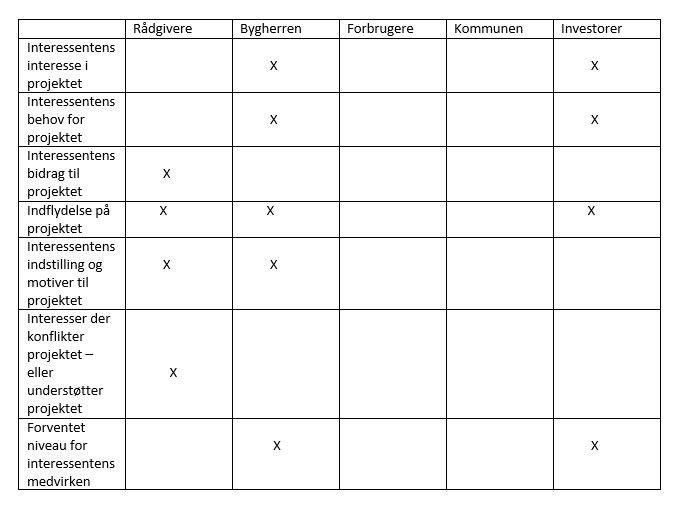
\includegraphics[width=0.80\textwidth]{billeder/IA1}
\caption{Tabel der viser de forskellige intersenters relevans for projektet.}
\label{fig:IA1}
\end{figure}

\subsection{Indflydelse}

\begin{itemize}
\item Bygherren/ejeren
\item Investorer og rådgivere
\item Kommunen
\item Forbrugere
\end{itemize}

Ved indflydelse menes der hvor relevant interessentens indflydelse er i forberedelsesarbejdet for et. Rækkefølgen er sat fra et til fire, hvor et har størst relevans. I dette tilfælde, er det i forhold til bygningsprojektet ved Strøybergs palæ.

I dette afsnit vil listen blive argumenteret for.

Ethvert byggeprojekt har en ejer, som i oftest tilfælde også er bygherren, altså en person eller organisation med et ønske om at opføre en konstruktion. Disse har sandsynligvis en lang række kriterier for projektet og vil gerne diktere retningen, som projektet skal tage. Desuden kan ejeren som regel nedlægge projektet til enhver tid, så længe alle er blevet betalt for det arbejde de måtte have udført. 

Hernæst er eventuelle investorer i projektet også yderst indflydelsesrige, idet projektet muligvis ikke er muligt at gennemføre uden deres økonomiske støtte til projektet. Investorerne kan altså også i og for sig nedlægge projektet, hvis det eventuelt ikke tager deres ønskede retning, ved at trække deres økonomiske støtte.

Desuden er rådgivere, ingeniører, arkitekter og økonomer også væsentlige brikker i den samlede forberedelsesfase. Uden deres hjælp ville alle større projekter ikke kunne gennemføres, idet der enten ville mangle beregninger, designs eller orden i økonomien.

Foruden ejeren og eventuelle investorer, spiller kommunen, hvori projektet skal gennemføres, også en stor rolle, eftersom den har dikteret en lokalplan, som skal følges, dog med mulighed for kompensation. Kommunen sætter med lokalplanen altså rammerne for projektet, hvormed de har den afgørende indflydelse i planlægningsfasen. Herefter er det usandsynligt, at kommunen har stor indflydelse, med mindre der bliver bygget uden for lokalplanens rammer. I sådan et tilfælde skal kommunen vurdere om der skal laves om eller om det er tilladt.
 
Forbrugerne har tilnærmelsesvis ingen indflydelse på projektet, idet de ikke ejer noget eller bidrager økonomisk til projektet.

\subsection{Medvirken}
Ved medvirken menes, hvor vigtig interessentens aktive medvirken er, i forhold gennemførelsen af projektet. Prioriteringen af interessenterne er valgt som følgende:

\begin{itemize}
\item Bygherren/ejeren
\item Investorer
\item Forbrugere og kommunen
\end{itemize}

Nedenfor vil denne prioritering argumenteres
Som højeste prioritet er det vurderet, at bygherren har den største medvirken til projektet. Grundlaget for, at projektet om tilbygningen til Strøybergs Palæ kan fuldføres, er først og fremmest, at der er et firma eller en privat person, som betaler for udførelsen af projektet. Bygherren er også den, som skal opføre projektet, efter de funktions- og designkrav, hvis der er en eventuel køber af slutproduktet. Det er derfor vigtigt, at bygherren er vel-informeret under hele projektet, da bygherren i første omgang ejer projektet. 

Bygherren har altså den største medvirken til projektet i den forstand, at uden en bygherre, ville projektet aldrig kunne realiseres. 

Herefter vurderes det, at investorerne har næsthøjeste prioritet i forhold til medvirken. Investorerne kan siges at være på sidekanten af projektet. De stiller ingen konkret arbejdsindsats til rådighed, men kan dog komme med mindre indvirkninger i mindre dele af projektet. Det er vigtigt, at de er involveret i hele projektet, da det er dem som skal investere i slutproduktet. 

Til sidst er der de eksterne interessenter, forbrugere og kommunen. Forbrugernes medvirken er ikke nødvendigt til opførelsen af projektet, men er interesseret i slutproduktet.  Kommunen har ikke nogen reel medvirken i projektet, men er interesseret i projektet som helhed, da det er en del af Aalborgs udvikling. Som nævnt i kapitel XX angående kommuneplanen, så er Aalborg på vej mod at være en kompetence by, hvilket betyder, at der vil være et større behov for kontorbygninger og boliger. Kommunen ser derfor positivt over for projekter som dette.

\section{Analyse opsamling}
Ser man på listerne, for henholdsvis indflydelse og medvirken, er de ens. Herved kan de konkluderes, at det øverste navn på listen har den afgørende stemme. Disse personer eller organisationer er hvad man kalder ressourcepersoner. Dette betyder samtidig, at beslutningen om ikke at gennemføre en tilbygning, som de tidligere ejere, TWT Aalborg, havde tænkt sig at gennemføre højst sandsynligt kom fra ejeren/bygherren. Eftersom det ikke har været muligt at skaffe informationer herom, er det kun muligt at spekulere i hvorfor de nuværende ejere, Calum A/S, ikke har valgt at gennemføre projektet. 

Den mest sandsynlige årsag ville være vedrørende økonomi. Måske har projektet vist sig at være for dyrt til at kunne betale sig. Herudover kunne det skyldes hensyntagen til naboer, hvis udsigt muligvis kunne blive blokeret af en eventuel fleretagesbygning. 

Om end usandsynligt, så er det muligt, at Calum A/S blot har anset tilbygningen for værende unødvendig.
